\documentclass[../main.tex]{subfiles}
\graphicspath{{figures/}{../figures/}}

\begin{document}

构造自动机类的数据类型和相关方法,
并检查状态转换是否正确,
运行
\begin{lstlisting}[language=python,numbers=none]
test = Automata('ab')
test.set_start_state(1)
test.add_final_states(2)
test.add_final_states(2)
test.add_transition(1,2,set(['a','b']))
test.add_transition(1,3,set('b'))
test.draw('../docs/figures/test_automata.pdf')
\end{lstlisting}
其中打印显示数据类型如下
\begin{lstlisting}
{1: {2: {'a', 'b'}, 3: {'b'}}}
states: {1, 2, 3}
start state:    1
final state:    {2}
transitions:
1->2 on 'a'
1->2 on 'b'
1->3 on 'b'
\end{lstlisting}

绘图结果如%
\cref{fig:testautomata}
\begin{figure}[H]
  \centering
  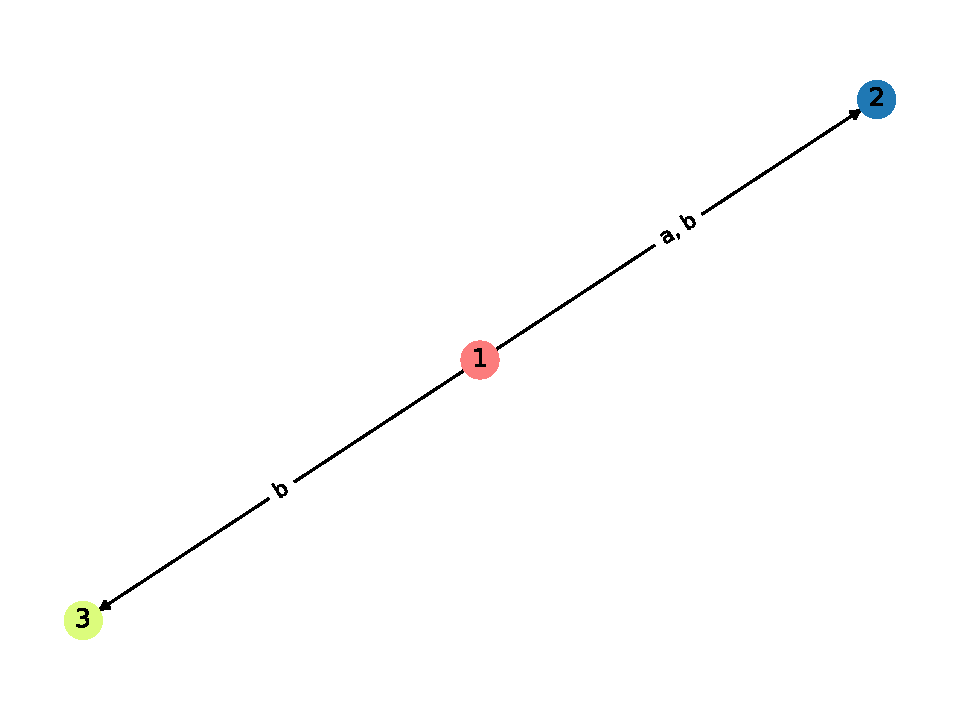
\includegraphics[width = 0.6\textwidth]{test_automata}
  %\missingfigure{automata}
  \caption{测试一个自动机}
  \label{fig:testautomata}
\end{figure}
\cref{fig:testautomata}蓝色点代表终态,红色代表初态,其他状态为绿色

\end{document}
